\documentclass[Report.tex]{subfiles}
\externaldocument[I-]{chapter_1_introduction}
\externaldocument[M-]{chapter_2_method}
\externaldocument[R-]{chapter_4_result}
\externaldocument[C-]{chapter_5_conclusion}
\externaldocument[RE-]{chapter_6_recognition}

\begin{document}
\chapter{Discarded Method}
\label{chap:Discarded Method}
\section{Description}
This chapter covers the methods tried but not included in the end result,
because they showed dissatisfactory results. This chapter is also organized
like Chapter~\ref{chap:Method}, but for component description please refer to the before mentioned chapter.

\section{Text Segmentation}
We tried to expand the original approach to be able to detect text with noise, natural images. We tried Stroke Width Transform first, then OpenCv scene text detection. We abandon both approach because of time constrain and difficulties of implementation. We decided therefore to focus on other part of the project first. 

\begin{flushleft}
  \subsubsection{Other Approach 1: Stroke Width Transform}
  We tried Stroke Width Transform to do Text Segmentation when original approach gave a decent result. It was original propose by Epstein et al 2010 \cite{epshtein_stroke_2010}. Since OpenCv do not have this implemented we tried to implement it ourself. Additional sources was used in our attempt to implement it\cite{werner_text_????, _c++_????, bunn_strokewidthtransform:_2018}. We was not able to finish this, but think we should mention it since we spend some time on it. The steps of Stroke Width Transform is as followed:
  \begin{enumerate}
    \item \textbf{Edge Detection and edge orientation(Done)}
    We need to have Edge image and orientation of the gradient image.
    Canny and Sobel was used in the original paper and other sources. This is simple since OpenCv have both Canny and Sobel implemented.
    \item \textbf{Stroke Width Transform(Done)}
    Here we had to do more. We have to find a line from a starting point and the angle. We was able to implement this part, but was some uncertainties. It only work on black text with white background. That is because the orientation(Sobel filtering) are dependent on it. The paper talk about doing a second pass with inverse image, but we decided to ignore it, in order to come farther in the algorithm.
    \item \textbf{Find Connected Component(Done)}
    In this point we are find connect component. The caveat here is the components need to be connected with regards to the Stride Length. We used 'One Component At A Time' algorithm to find all the different components. This part we was able to finish.
    \item \textbf{Exclude noise and find letters(not Done)}
    Since Stroke Width Transform tend to make a lot of noise. The obvious one is making single lines. This part are suppose to exclude this noise and at the same time exclude anything that is not a letter.The theory is, since letter and text all usually have the same stroke width, we can use this information do estimate what is letter and what is not. We was not able to finish this part.
    \item \textbf{Find lines/words(not Done)}
    Was not able to get to this part, but ideal it will combine letters to a single line or words.
  \end{enumerate}
  In cases where the image have a lot of non text object, it will work fine with it. We ended up discarding this approach since it was to time consuming and decided on working on simple approach first.
\end{flushleft}

\begin{flushleft}
  \subsubsection{Other Approach 2: OpenCv Scene Text Detection}
  OpenCV have it own Text Scene Detection. The approach of this algorithm is to detect text in scene using Classifier and Components Tree, propose by Lukás Neumann \& Jiri Matas \cite{neumann_real-time_2012}. Since we already discarded Stroke Width Transform to focus on simple approach, we decided not use it. We had some problem to get propel result as well.
\end{flushleft}

\subsection{Used in end result}
Since we had problem on getting with both approach 2 and 3 we decided on approach 1. It gave us ideal result on most images, but have some problem in images with non text objects.

\section{Preprocessing}
\subsection{Find rotation}

\begin{flushleft}
  \textbf{Approach: Hough Transform} \\
  \href{https://en.wikipedia.org/wiki/Hough_transform}{Hough transform} is a
  well known algorithm to find lines, its approach is to see if it can
  align some threshold of pixels on one straight line. To help with this
  process we will do a simple edge detection algorithm on the image before
  running it through the Hough Transform. \par
  Bellow, the steps needed to perform this approach are mentioned.

  \begin{enumerate}
    \item \textbf{Edge detection}
    Too make the Hough transform perform better we want to remove unnecessary
    noise. Canny edge detection algorithm is a robust and fast solution for
    this.
    \item \textbf{Line detection}
    Now perform the actuall Hough Transform.
    \item \textbf{Rotate image}
    Lastly we need to rotate the image according to the lines from the Hough
    Transform.
  \end{enumerate}
\end{flushleft}

\section{Classification}
\label{sec:Discarded Method:Classification}

\begin{flushleft}
  \textbf{Deep Neural Network} \\
  Multilayer perceptron neural networks are relatively straight
  forward to code, however the challenging part is to decide on good
  hyper-parameters and to not overfit our network. \par
  Research has shown that the choices of parameters can have huge effects on
  the error rate through empirical testing. As empirical testing has shown that
  some combinations of parameters are better than others, we will also use the
  same method to find decent values on several of the hyper-parameters. More on
  this bellow, where a short description of the hyper-parameters follow. \par
  One obvious disadvantage we might face by using MLP is that slight spatial
  change on where in the image the characters are located, might lead to
  characters classified differently. This is because there is no spatial
  connections on a MLP.
\end{flushleft}

\begin{figure}[H]
  \centering
  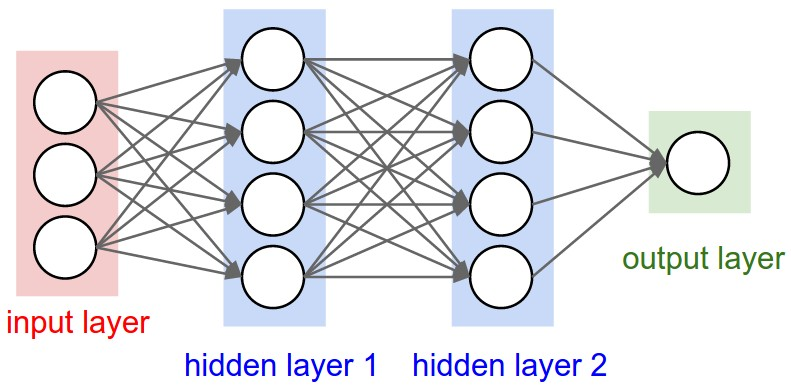
\includegraphics[height=4cm]{res/neural_net2.jpeg}
  \caption{MLP Neural network \href{http://cs231n.github.io/neural-networks-1/}{Source}}
  \label{fig:neural_net2}
\end{figure}

\begin{flushleft}
  \textbf{Hyper-parameters}
  \begin{itemize}
   \item{Number of hidden layers}
   \begin{itemize}
    \item{Layers decide how well the software can define the decision borders.
    Hence increase in layers can have a positive effect, there are also cons with
    the amount of layers. The more layers, the greater the computational power
    needed to train the system. We will be using the empirical method to decide
    how many layers we need}
   \end{itemize}
   \item{Number of nodes in each hidden layer}
   \begin{itemize}
    \item{Nodes in each hidden layer has the same effect as the number of hidden
    layers, hence the same applies for this hyper-parameter. }
   \end{itemize}
   \item{Activation functions}
   \begin{itemize}
    \item{The activation function decides which combination of nodes, with their
    signals, are allowed to propagate through the network. Here we will be using
    the \textit{rectified linear unit} (RELU) activation function. This is an
    activation function that allows propagation if the signal is positive,
    otherwise it will forward a zero. The reason for choosing this activation
    function is because this function handles the \textit{vanishing gradient
    problem} better than sigmoid and a tanh activation functions. More on
    vanishing gradient problem under ``optimization function''.}
   \end{itemize}
   \item{Loss function}
   \begin{itemize}
    \item{The loss function describes how far off the predicted class of the
    character is from the real class. In our case since we have multiple
    classes and we are going to use \textit{softmax regression} as the output
    layer, we also will be using the \textit{cross-entropy loss function}.}
   \end{itemize}
   \item{Optimization function}
   \begin{itemize}
    \item{The backpropogation will train the weights by Gradient Decent
    Optimization. However as training with several thousand examples, and then
    optimizing the weights and run the training process, is too costly resource
    wise, we will have to implement the \textit{mini-batch gradient decent
    optimizations}. Same principle as gradient decent optimization, but this way
    we will find the gradient decent for each batch. As long as these batches are
    randomly chosen, and the sizes are large enough, (we will be using 100 as
    batch size), these will represent the entire dataset well enough.}
   \end{itemize}
   \item{Learning rate}
   \begin{itemize}
    \item{Learning rate is a scalar that decides how large the steps towards
    the gradient minimum will be, for the weights. Choosing too small of a
    learning-rate we might risk not reaching the bottom of the graph, we also
    might get stuck in a local minimum. Choosing too large of a learning rate
    we might risk never settle down on a minimum. \par
    For the learning rate we will be using the empirical method too.}
   \end{itemize}
   \item{Initialization of the weights and biases}
   \begin{itemize}
    \item{Initialization of the weights also seems to be of importance,
    researchers have found out. This is obvious, as for example setting all the
    weights to zero, would of course lead to a network with very few active
    nodes. \par
    We will be using the initialization of zeros for the biases, not any
    apparent reason. Based on our research, it seems people have gotten decent
    results when using this initialization. For the weights we will be using a
    gaussian distribution, mean=0, standard deviation=1. Again this is also
    something that we have read should be a good initialization for the weights,
    no other reason.}
   \end{itemize}
   \item{Number of epochs}
   \begin{itemize}
    \item{Number of epochs are only relevant when we have a small number of
    dataset. When we have a small dataset we might want to run the software on
    the same dataset several times. This might result in overfitting the software
    to the dataset, therefore it is really important to be careful of the number of
    epochs, in cases with small datasets.}
   \end{itemize}
  \end{itemize}
\end{flushleft}


\section{Datasets}


\end{document}
